\chapter{Fournisseurs}

\section{Fournisseurs}
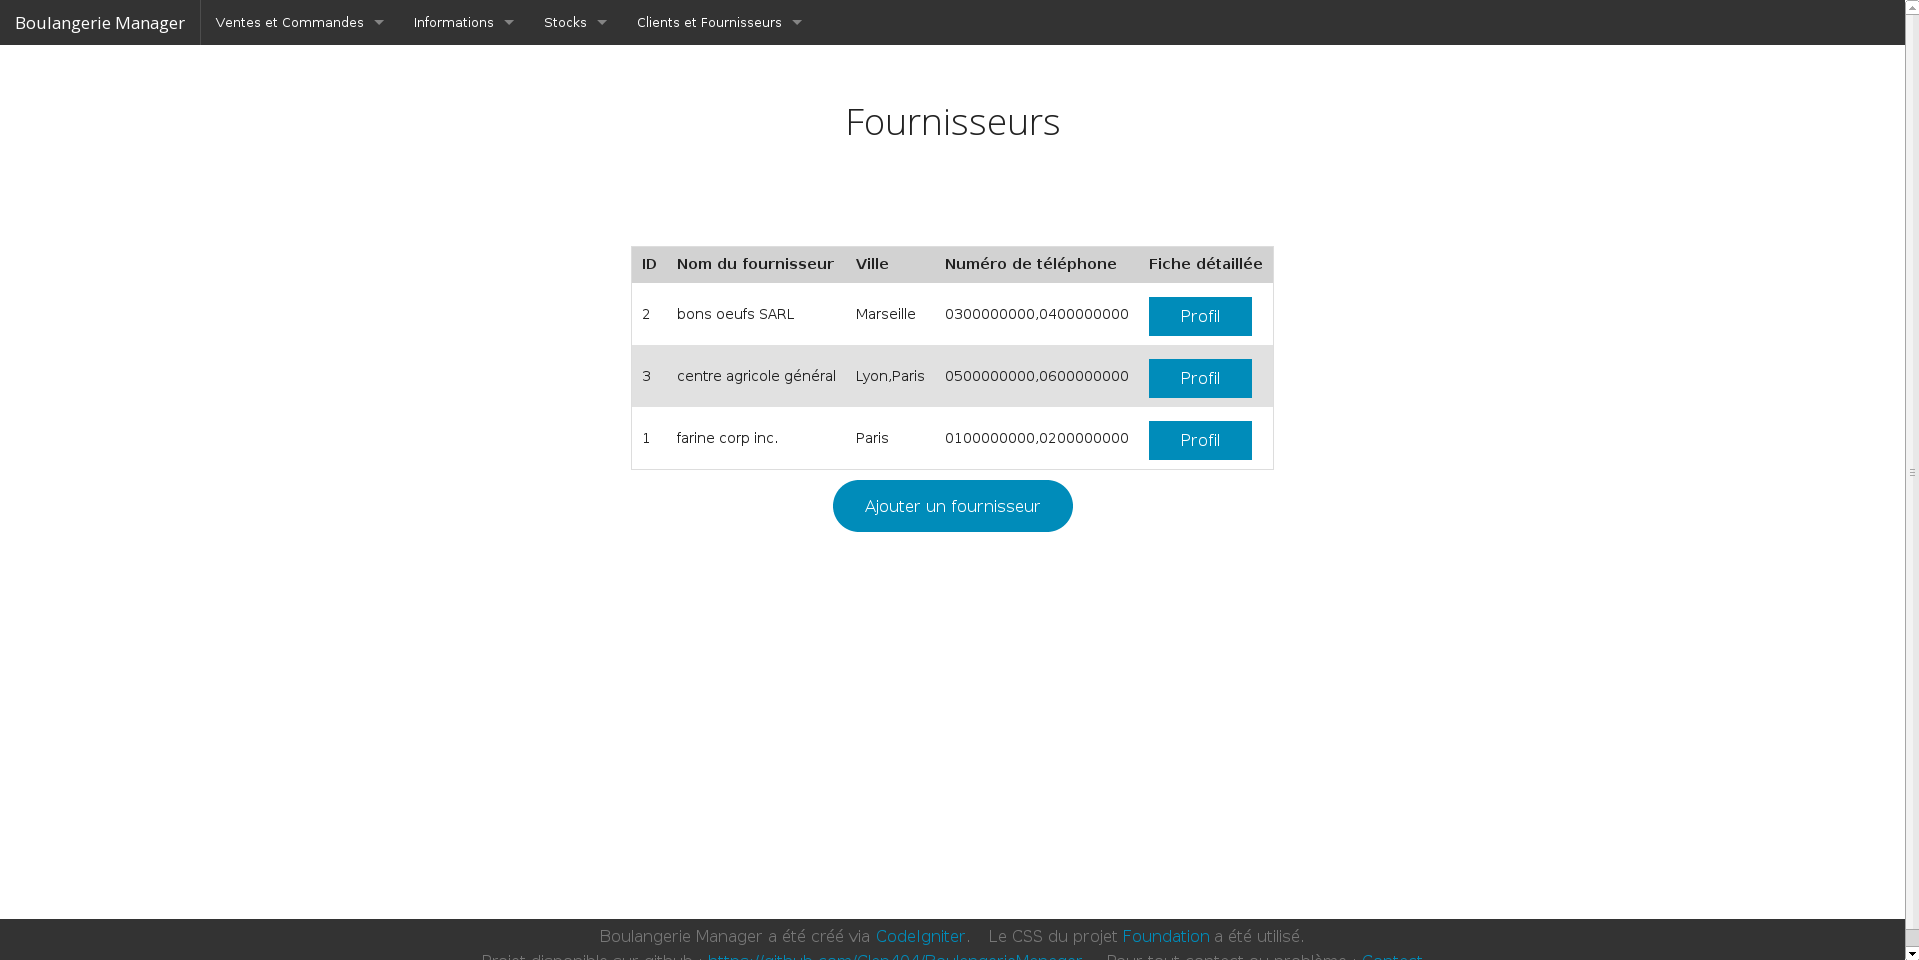
\includegraphics[scale=0.30]{fournisseur1.png}\\
Cette page liste les fournisseurs par ordre alphabétique. Pour chaque fournisseur, sont
affichés le nom, les villes depuis lesquelles livre le fournisseur et
les numéros de téléphone.

\paragraph{}
Le bouton "Profil" permet d'accéder à la fiche détaillée de chaque fournisseur.

\subsection{Ajout d'un fournisseur}
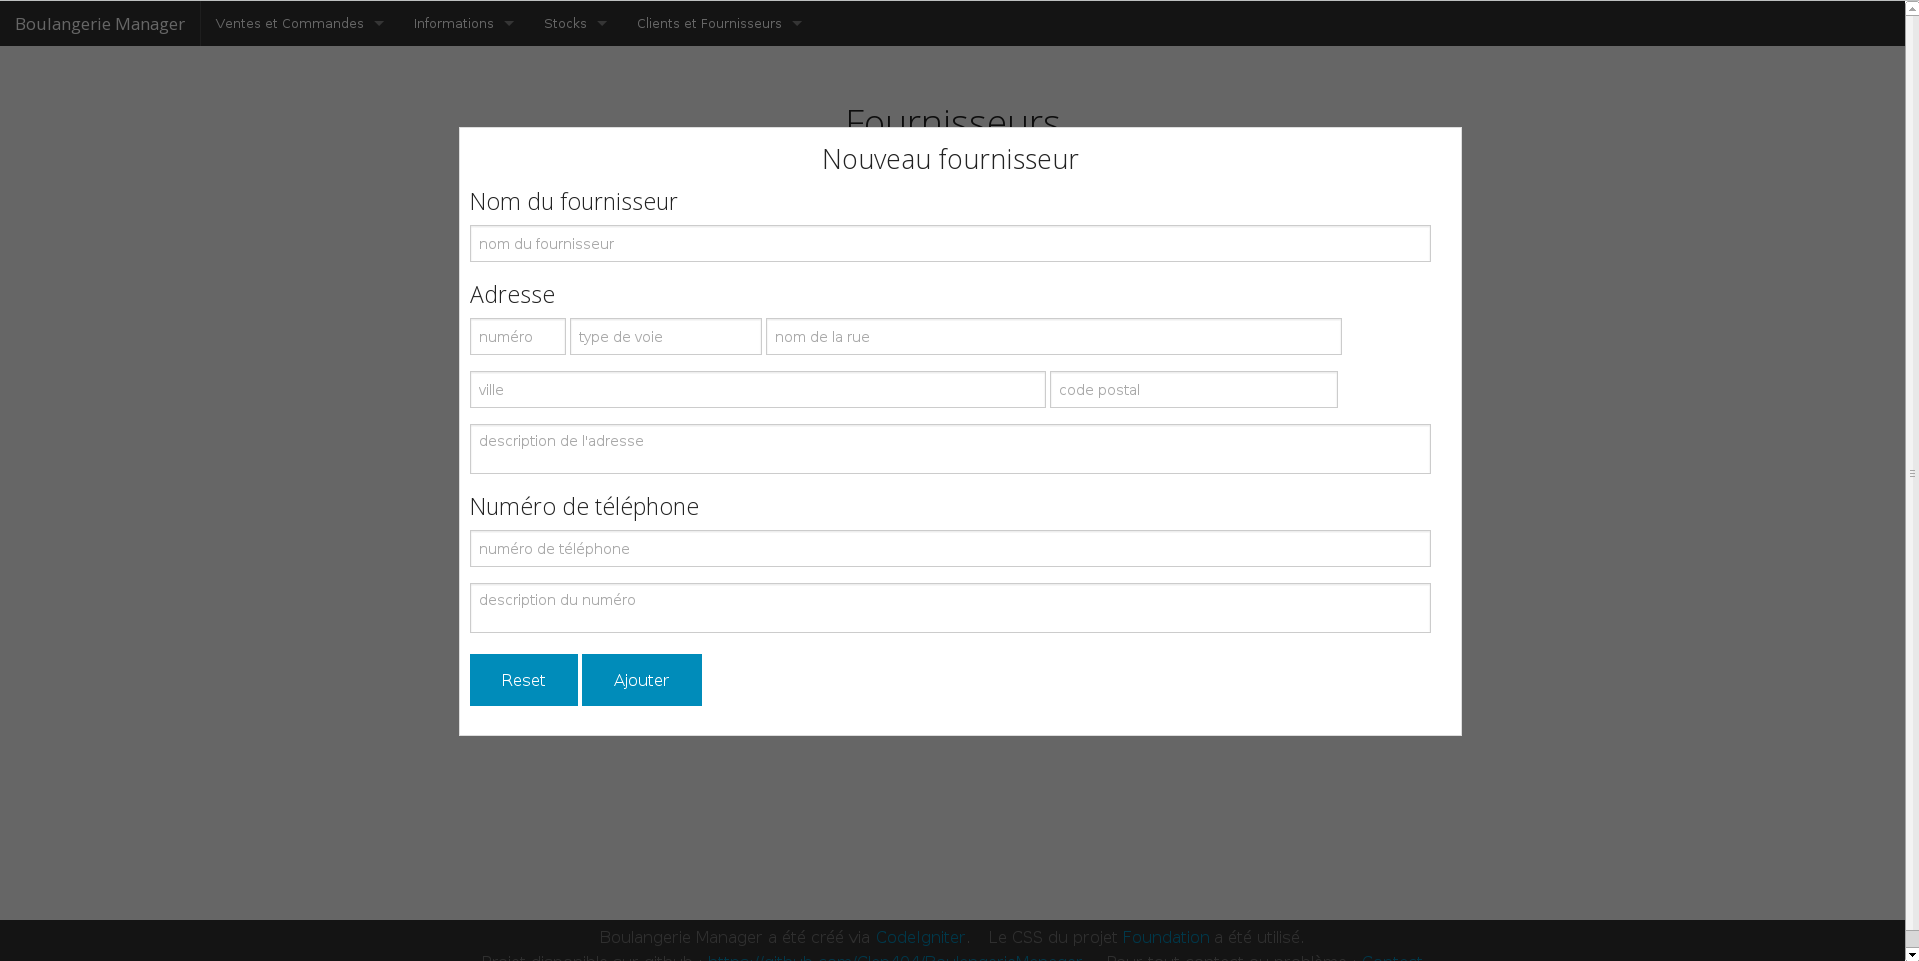
\includegraphics[scale=0.30]{fournisseur2.png}\\
Sur la page "Fournisseurs", la liste de fournisseurs est suivie d'un bouton
"Ajouter un fournisseur". Un clic sur ce bouton fait apparaître un formulaire au
premier plan, semblable au formulaire d'ajout de clients.

\section{Profil}
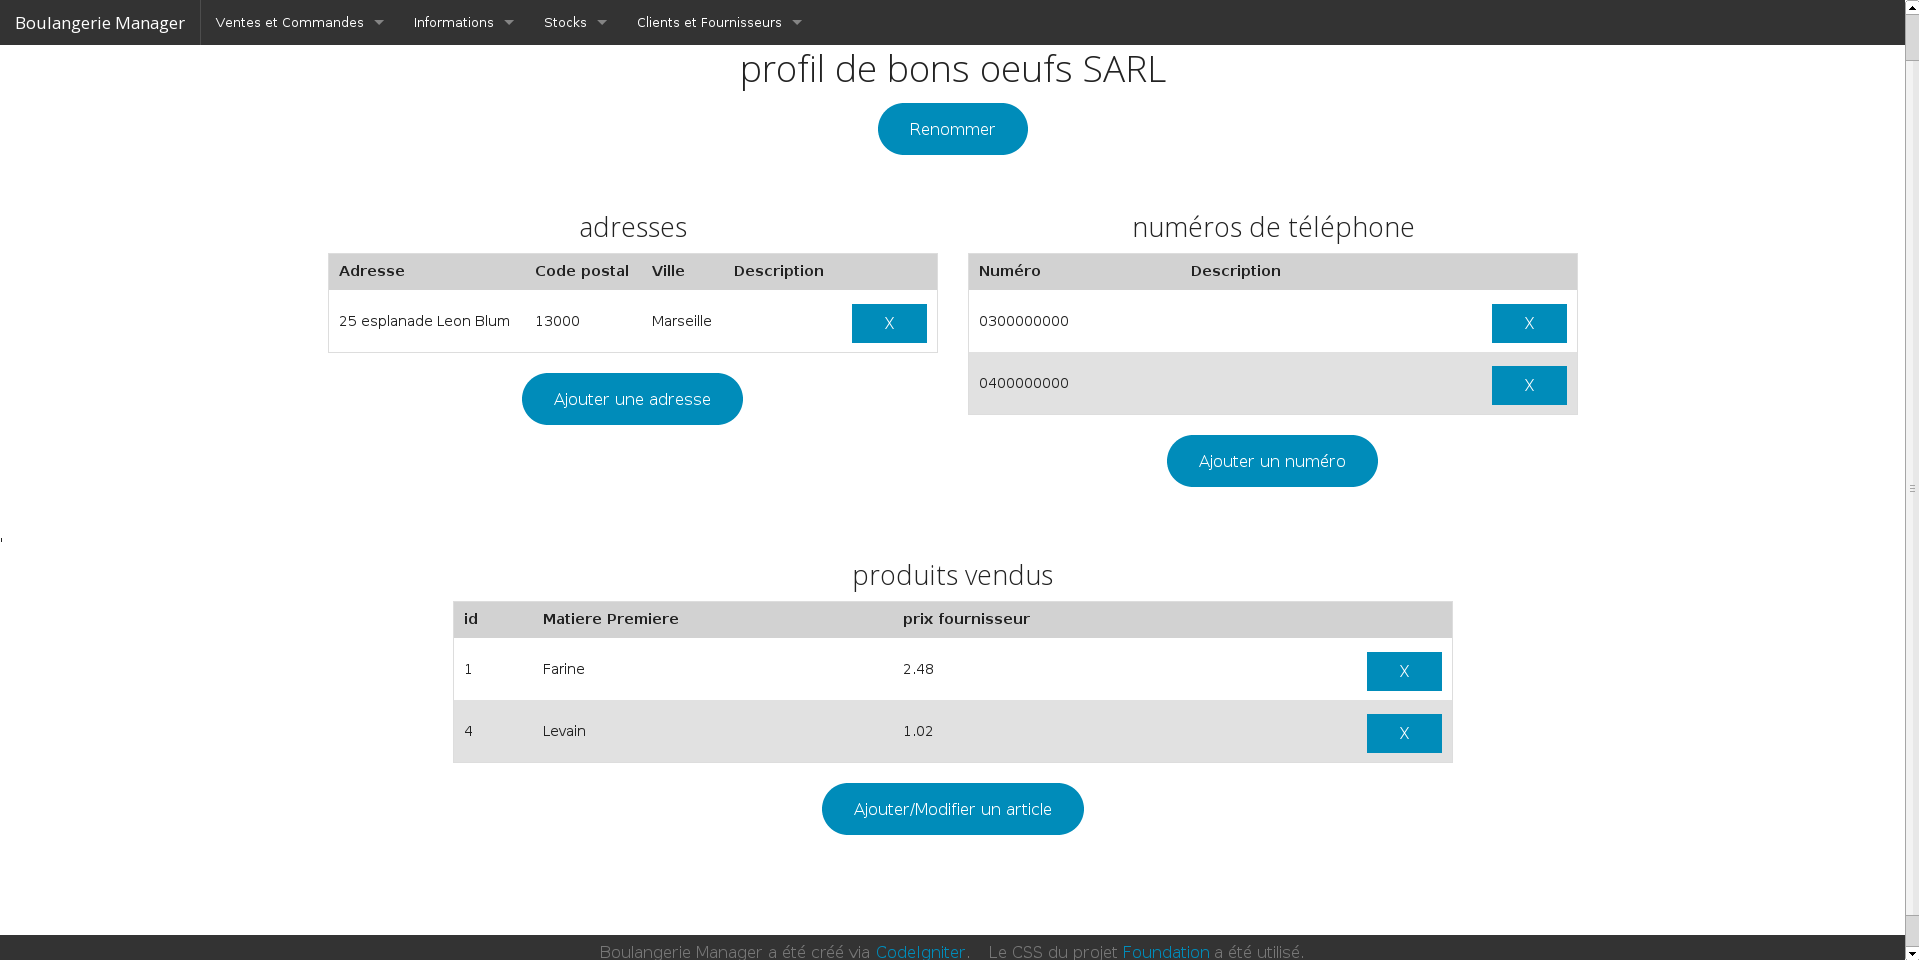
\includegraphics[scale=0.30]{fournisseur3.png}\\
La page de profil est composée de quatre champs d'information :

\begin{enumerate}
  \item Le nom du fournisseur
  \item Les adresses du fournisseur
  \item Les numéros de téléphone du fournisseur
  \item Les produits vendus par le fournisseur
\end{enumerate}

\subsection{Ajout d'informations sur les fournisseur}
Chaque champ d'information est accompagné d'un bouton permettant l'ajout d'informations.
Un clic sur l'un de ces boutons fait apparaître le formulaire d'ajout
d'information associé.

\paragraph{}
Comme pour les clients, chaque champ d'information sur la page de profil
des fournisseurs dispose
d'un bouton permettant l'ajout d'informations.

\paragraph{}
Le bouton "Ajouter/Modifier un article" permet d'ajouter un produit vendu par le
fournisseur avec le prix pratiqué par ce fournisseur mais aussi de modifier le
prix d'un produit déjà ajouté.

\paragraph{}
Notez que seules les matières premières doivent
d'abord être ajoutées via l'onglet "Matières premières" dans la section "Stock"
pour pouvoir être ajoutées au profil d'un fournisseur.

\subsection{Suppression d'informations sur les fournisseurs}
Les lignes pouvant être supprimée possèdent
un bouton avec une croix. Un clic sur ce bouton supprime directement
l'information de la mémoire.

\paragraph{}
Les listes "Adresses" et "Numéros de téléphone" doivent toujours contenir au
moins une entrée. Par conséquent, le bouton de suppression de fonctionnera pas
si la liste ne contient plus qu'une entrée.
